\def\year{2016}\relax
%File: formatting-instruction.tex
\documentclass[letterpaper]{article}
\usepackage{aaai16}
\usepackage{times}
\usepackage{helvet}
\usepackage{courier}

\usepackage[T1]{fontenc}
\usepackage{ae,aecompl}
\usepackage{amsfonts}
\usepackage{amsmath}
\usepackage{amsthm}
%\usepackage[table,xcdraw]{xcolor}
% Use the postscript times font!
\usepackage{graphicx}
\usepackage{bbm}
\usepackage[usenames]{color}
\usepackage{wrapfig}

\newcommand\meir[1]{\textcolor{red}{meir: #1}}
\newtheorem{definition}{Definition}
\newcommand{\AG}{{\tt ActionGenerator}}
\newcommand\sysrep[1]{{\tt SystemRepair(#1)}}
\newcommand{\notrep}{\overline{Repaired}}
\newcommand{\myopic}{{\tt Myopic-BRP}}
\newcommand{\cost}{\textit{cost}}
\newcommand{\COMPS}{\textit{COMPS}}
\newcommand{\SD}{\textit{SD}}
\newcommand{\OBS}{\textit{OBS}}
\newcommand{\planbased}{{\tt Plan-based-BRP}}

\frenchspacing
\setlength{\pdfpagewidth}{8.5in}
\setlength{\pdfpageheight}{11in}
\pdfinfo{
/Title (Implementing Troubleshooting with Batch Repair)
/Author (Roni Stern, Meir Kalech and Hilla Shinitzky)}
\setcounter{secnumdepth}{0}  
 \begin{document}
% The file aaai.sty is the style file for AAAI Press 
% proceedings, working notes, and technical reports.
%
\title{Implementing Troubleshooting with Batch Repair}
\author{Roni Stern \and Meir Kalech \and Hilla Shinitzky \\
Ben Gurion University of the Negev\\
Be'er Sheva, Israel \\
}
\maketitle
\begin{abstract}
Recent work has raised the challenge of efficient automated troubleshooting in domains where repairing a set of components in a single repair action is cheaper than repairing each of them separately. This corresponds to cases where there is a non-negligible overhead to initiating a repair action and to testing the system after a repair action. In this work we propose several algorithms for choosing which batch of components to repair, so as to minimize the overall repair costs. Experimentally, we show the benefit of these algorithms over repairing components one at a time. % (and not as a batch).
\end{abstract}




\section{Introduction}
% Troubleshooting, but have repair overhead
Troubleshooting algorithms, in general, plan a sequence of actions that are intended to fix an abnormally behaving system. Fixing a system includes repairing faulty components. Such repair actions incur a cost. These costs can be partitioned into two types of repair cost. The first, referred to as the {\em component repair cost}, is the cost of repairing a component. The second, referred to as the {\em repair overhead}, is the cost of preparing the system to perform repair actions (e.g., halting the system) and the cost of testing the system after performing a repair action.

% Thus, batch repair makes sense. Introducing BRP
This paper considers the case where the repair overhead is not negligible and is potentially more expensive than a component repair cost (of a single component). Therefore, it may be more efficient to repair a batch of components in a single repair action. We call the problem of choosing which batch of components to repair the Batch Repair Problem (BRP). BRP is an optimization problem, where the task is to minimize the {\em total repair costs}, which is the sum of component repair costs and costs due to repair overheads incurred by repair actions performed until the system is fixed.

% Terminology : fix and repair
Note that in this paper we use the term  ``fix'' when referring to the entire system and term ``repair'' for a single or a set of components.  Thus, 
to {\em fix} the system one needs to {\em repair} components, and a system is only fixed if it returned to its nominal behavior.

%\meir {i think we should say something like this explicitly: We consider, in this paper, two kinds of repair costs. The first is the cost of the replaced component. The second is the cost of the system check after repairing some component(s). We assume in this paper that the system check cost is more expensive than the cost of rearing a single component, and therefore it is be more efficient to repair multiple components before operating a system check. }

%Such repair actions incur various costs beyond the cost of repairing the actual components. Such costs can include the overhead of initiating a repairing process, e.g., halting an assembly line, as well as the cost of testing the system after a repair to verify that problem has been fixed. We call these overhead cost the {\em repair overhead}.\footnote{In addition to the repair overhead, one may also consider the cost of the system not being operational~\cite{friedrich1992choosing}.} We study the problem of how to choose which components to repair, so as to minimize the total costs of repairing a system: the repair overhead costs incurred until the system is fixed plus the cost incurred for repairing the individual components.

% Previous work did not try to batch-repair. We need a cost-effective solution that does.
Most previous work assumed that components are repaired one at a time \cite{heckerman1995decision,friedrich1992choosing,Nyberg12,Torta14}. This approach can be wasteful for BRP. For example, if a diagnosis engine infers that multiple faulty components need to be repaired to fix the system, then it would be wasteful to repair these components one at a time since each repair action incurring its repair overhead. Instead, an efficient BRP algorithm would repair all the faulty components in a single repair action. More generally, we expect an intelligent BRP algorithm to consider to repair overheads and the component repair costs when deciding which components to repair. 
% weigh the cost of repairing batches of components as well as the repair overhead. %Some discussion on repairing multiple components together was done in prior work on self healability~\cite{cordier2007selfHealability}.

% Why is BRP hard.
Due to the repair overhead, repairing a single component, even if it is the component most likely to be faulty, can be wasteful. This is especially wasteful in cases where all the found diagnoses consist of multiple faulty components, thus suggesting that repairing a single component would not fix the problem. Alternatively, one may choose to repair the components in the single most likely diagnosis. This may also be wasteful, especially if there are several diagnoses which have similar likelihood. It might be worthwhile to repair, in a single repair action, a set of components that ``covers'' more than a single diagnosis. This may reduce the number of repair actions until the system is fixed, thus saving repair overhead costs. The downside in this approach is that healthy components may be repaired, increasing the overall repair costs.

 %the component repair costs can be high, as more healthy components may be repaired.


\begin{figure}{}%{4cm}
\begin{center}
  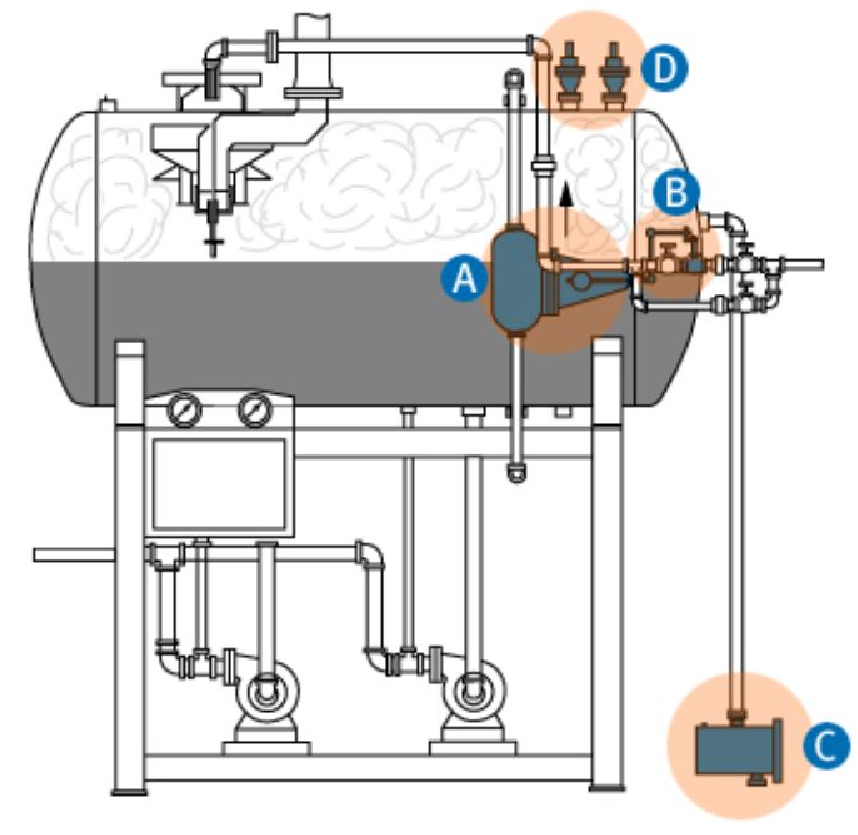
\includegraphics[width=0.9\columnwidth]{figures/system_example.pdf}
  \caption{An example where repairing components one at a time is wasteful.}
  \label{fig:simple-example}
\end{center}
\end{figure}
%
%\begin{figure}%
%\centering
%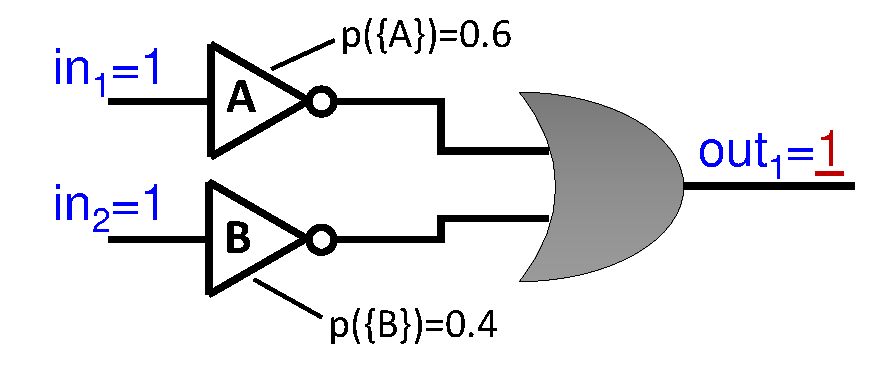
\includegraphics[width=0.6\columnwidth]{simple-example.pdf}%
%\caption{An example where repairing components one at a time is wasteful.}% If $cost_{repair}=10$ and $cost_A=cost_b=1$, the best repair action is to repair $A$ and $B$ together.}%
%\label{fig:simple-example}%
%\end{figure}
%
For example, consider the boiler tank system scheme made by Warren Controls, Inc. described in Figure~\ref{fig:simple-example}. When demand for water reduces the liquid level in the tank, the float cage ($A$) opens the lever valves ($B$) to supply intake water to the tank and closes it when the water reaches the desired level. Component $C$ is an overflow trap which collects and relieves condensate overflow. Component $D$ includes two vacuum breakers which are opened to relieve the tank with outside air to prevent vacuum pressures in the tank.

Assume additional water is required but the level of the water does not increase. There are two possible diagnoses: either the float cage $A$ is faulty or the lever valve $B$ is faulty. Assume that the probabilities of $A$ and $B$ to be faulty are given by the manufacturer and are 0.06 and 0.04, respectively. Since only these diagnoses can explain the problem, the normalized probability of $A$ to cause the problem is 0.6 and that of $B$ is 0.4. There are three possible repair actions: to repair $A$, to repair $B$, and to repair $A$ and $B$. Assume the repair cost of each component is 5\$ but the repair overhead is 50\$, due to the cost of opening the tank and boiling the water. If $A$ is repaired, there is a 0.4 chance that the system would not be fixed and another repair action would be needed (repairing $B$). Thus, the expected total repair cost of repairing $A$ first is $0.4\cdot(5+50)+5+50=77$. Similarly, the total repair cost for repairing $B$ first is $0.6\cdot(5+50)+5+50=88$. The best option is thus to repair $A$ and $B$ together in a single repair action, incurring a total repair cost of $5+5+50=60$.


%the repair overhead is larger than the cost of repairing a single component. \meir{i do  not understand the last sentence. the reason that repairing all the components is inefficient is due to the high cost of the components and not because the cost of the overhead.}

%Alternatively, one may consider repairing all the components in a single diagnosis, e.g., the most probable diagnosis. This too, however, may be inefficient in cases where the repair overhead is larger than the cost of repairing a single component. \meir{i do  not understand the last sentence. the reason that repairing all the components is inefficient is due to the high cost of the components and not because the cost of the overhead.} For example, consider the system depicted in X \meir{very important to add an example}

%\meir {i think we should say something like this explicitly: We consider, in this paper, two kinds of repair costs. The first is the cost of the replaced component. The second is the cost of the system check after repairing some component(s). We assume in this paper that the system check cost is more expensive than the cost of rearing a single component, and therefore it is be more efficient to repair multiple components before operating a system check. }

%(MEIR: obviously the next two paras should be modified. you can say that previous work proposed...)
% We first show how to optimally do this
%\meir{
%Recent work~\cite{stern2015repair} proposed two high-level approaches to solve BRP: as a planning under uncertainty problem, or as a combinatorial optimization problem. When modeling BRP as a planning under uncertainty problem the task is to find a {\em repair policy}, mapping a state of the system to the repair action that minimizes the expected total repair costs. This approach, while attractive theoretically, quickly becomes not feasible in non-trivial scenarios.}

In this work we model BRP as a combinatorial optimization problem, searching in the combinatorial space of possible repair actions for the best repair action. There are two challenges in implementing this approach: (1) how to measure the quality of a repair action, and (2) how to efficiently search for the repair action that maximizes this measure. There are many efficient heuristic search algorithms in the literature, and thus we focus on the first challenge --- developing intelligent heuristics for estimating the merit of a repair action.


%We analyze what should the best repair action be and propose several heuristics for choosing the best repair actions in practice.

%Both approaches are unfeasible in large systems, as the number of repair actions would be just too large. We propose a range of possible relaxations, considering only a subset of the possible repair actions, to tradeoff runtime for solution quality.
%\meir{We first propose an optimal algorithms by modeling the planning problem as Markov Decision Process (MDP). The optimal algorithm guarantees repairing the system with minimal cost but its runtime is exponential. We propose then some relaxations to reduce the exponential runtime of the MBD and the MDP.}



The contributions of this work are practical. A range of heuristic objective functions are proposed and analyzed, and we evaluate their effectiveness experimentally on a standard benchmark. A clear observation from the results is that indeed considering batch repair actions can save repair cost significantly and that intelligent heuristics are crucial in saving repair costs.% Moreover, the most effective heuristics provide a tunable tradeoff between computation time and resulting repair costs.

%This lays the foundation for future work that would examine the effectiveness of the range of suboptimal solvers we propose in practical domains.


\section{Problem Definition}
Next, we provide background required for defining the batch repair problem we address. %and definitions required for describing the batch repair algorithms we propose.
% Classical input
Following standard model-based diagnosis (MBD) terminology, we denote by $\COMPS$ and $\OBS$ the components in the system and the observed system behavior, respectively. $\SD$ describes the behavior of the diagnosed system, and in particular the behavior of each component. The term {\em behavior mode} of a component refers to a state of the component that affects its behavior. $\SD$ describes for every component one or more behavior modes. For every component, at least one of the behavior modes must represent the nominal behavior of the component. The normal mode is often described by the clause $h(C_i) \rightarrow \varphi_{C_i}$, where $C_i\in \COMPS$, $h(C_i)$ is a predicate stating that $C_i$ is healthy, and $\varphi_{C_i}$ describes the nominal behavior of $C_i$. For instance, the nominal behavior of the lever valve (component $B$ in Figure \ref{fig:simple-example}) is to be opened once the float cage opens it, while an abnormal behavior can be stuck open or close.

A {\em batch repair problem} (BRP) arises when the assumption that all components are normal is not consistent with the system description and observations. Formally,
\[ \SD \wedge \OBS \wedge \bigwedge_{C\in \COMPS} h(C) ~~~ \text{is not consistent} \]

% Health assignment
%A health assignment $\omega$ is an assignment of {\em behavior modes} to components. Let $\omega^{(+)}$ be the set of components assigned a nominal (i.e., healthy) behavior mode and $\omega^{(-)}$ be the set of components assigned one of the other modes.
A mode assignment $\omega$ is an assignment of {\em behavior modes} to components. Let $\omega^{(+)}$ be the set of components assigned a nominal (i.e., normal) behavior mode and $\omega^{(-)}$ be the set of components assigned one of the other modes.


%\meir{i think that the word "health" here is a little bit confusing since you do not mean that all assignments are in mode health. maybe "satisfying assignment"? Roni: we used this term in the duality paper, so I assumed it is standard? anyhow, I changed to mode so I'll have the letter h for heuristic}

\begin{definition}[Diagnosis]
A mode assignment $\omega$ is called a diagnosis if $\omega \wedge \OBS \wedge \SD$ is satisfiable.
\end{definition}

In the example shown in Figure \ref{fig:simple-example}, assuming that all components are healthy under the observation that the water level is decreased is not consistent. Then a possible diagnosis is that components $C$ and $D$ are healthy, while either $A$ or $B$ are in an abnormal mode. For instance, the lever valve ($B$) is stuck close.

\noindent In such a case, at least one component must be repaired.

\begin{definition}[Repair Action]
A repair action can be applied to any subset of components and results in these components becoming normal. Applying a repair action to a set of components $\gamma$ is denoted by Repair($\gamma$).
\label{def:repairAction}
\end{definition}
Definition~\ref{def:repairAction} assumes that repair actions always succeed, i.e., a component is normal after it is repaired. %[Roni: TODO: discuss how to relax this assumption later in the paper.]

% What happens after a repair action
After a repair action, the system is tested to check if it has been fixed.
We assume that the system inputs in this test are the same as in the original observations ( $\OBS$ ). The observed system outputs are then compared to the expected system outputs of a healthy system. Thus, the result of a repair action is either that the system is fixed, or a new observation that may help choosing future repair actions.


%\meir{to make the last sentence more accurate i propose to add: and all its subsets are not diagnoses.}
%Note that the notion of kernel diagnosis is only relevant in strong fault models (SFM) as oppose to weak fault model (WFM). \meir{you can say that in wfm kernel=minimal, while in sfm kernel is subset of minimal. Roni: done later int he apepr}
%Using MBD to Solve BRP \meir{???}


% *** Define a diagnosis engine and what it returns ***
A model-based diagnosis engine (MBDE) accepts as input $\SD$, $\OBS$, and $\COMPS$ and outputs a set of diagnoses $\Omega$. Although a diagnosis is consistent with $\SD$ and $\OBS$, it may be incorrect. A diagnosis $\omega$ is {\em correct} if by repairing the set of components in $\omega^{(-)}$ the system is fixed. Some diagnosis algorithms return, in addition to $\Omega$, a measure of the likelihood that each diagnosis is {\em correct}~\cite{williams2007conflict,abreu2011simultaneousDebugging}. Let $p: \Omega \rightarrow [0,1]$ denote this likelihood measure. We assume that $p(\omega)$ is normalized so that $\sum_{\omega\in\Omega} p(\omega)=1$ and use it to approximate the probability that $\omega$ is correct.


% Light at the end of the tunnle
A common way to estimate the likelihood of diagnoses, assumes that each component has a prior on the likelihood that it would fail and component failures are independent. Therefore, if $p(c)$ represents the likelihood that a component $c$ would fail then diagnosis likelihood can be computed as
\begin{equation}
\displaystyle p(\omega)=\frac{\prod_{c\in\omega^{-}} p(c)}{\sum_{\omega'\in\Omega}{\prod_{c\in\omega'^{-}} p(c)}}
\label{eq:likelihoods}
\end{equation}
where the denominator is a normalizing factor. %If diagnoses likelihoods are computed according to Equation~\ref{eq:likelihoods}, then they can be computed ``online'' and there is no need to represent them explicitly.  %\meir{i dont know what you mean here online.} [[Roni:  not sure about the English of the last sentence]] [[Roni: removed the unclear part]]
We assume in the rest of this paper that diagnoses likelihoods are computed according to Equation~\ref{eq:likelihoods}. Other methods for computing likelihood of diagnoses also exist~\cite{mengshoel2010probabilistic}.

% Repairing incurs a cost
Repairing a set of components incurs a cost, composed of a repair overhead and component repair costs. The repair overhead is denoted by $\cost_{repair}$, and the component repair cost of a component $c\in \COMPS$ is denoted by $\cost_{c}$.

%The repair overhead correspond to the system costs involved in initiating a repair action, e.g., stopping an assembly line to take out the components to be repaired, as well as the cost of testing the system's behavior after the repair action was performed. The component repair cost $cost_{C_i}$ correspond to the actual cost of repairing $C_i$, e.g., the cost of replacing the faulty parts of $C_i$.

%\meir{the notations are confusing. you have two types of costs so name both cost. the overhead can be $cost_{ovrhd}$ and the cost of component $cost_{C_i}$ Roni: modified as you said +-}

\begin{definition}[Repair Costs]
Given a set of components $\gamma\subseteq \COMPS$, applying a repair action Repair($\gamma$) incurs a cost:
\[ \cost(Repair(\gamma)) = \cost_{repair} + \sum_{c\in \gamma} \cost_{c} \]
\end{definition}
We assume that all repair costs are positive and non-zero, i.e., $\cost_{repair}>0$ and $\cost_{c}>0$ for every component $c \in \COMPS$. As defined earlier, the task in BRP is to fix a system with minimum total repair cost.

%We denote by {\em total repair cost} this sum of repair costs incurred until the system is healthy,
%and call the problem of minimizing the total repair cost the Batch Repair Problem (BRP).

As shown in Figure~\ref{fig:simple-example}, an efficient BRP solver should consider the possibility of repairing a set of components in a single repair action. Thus, the potential number of repair actions is %exponential in the number of components, in particular the power set of the components
$2^{|\COMPS|}$. Therefore, from a complexity point of view BRP is an extremely hard problem.


%BRP differs from other troubleshooting problems in the assumption that $C_{repair}>0$. \meir{i do not agree. f.i. heckermann assumed this. the different is the multiple component repair.} This assumption entails that an algorithm for solving BRP should consider the possibility of repairing a set of components in a single repair action. This causes the potential number of repair actions to be exponential in the number of components, in particular the power set of the components $2^{|COMPS|}$. Thus, from a complexity point of view BRP is an extremely hard problem.

%[[Roni: is the paragraph above redundant?]] \meir{no it is ok}
%\meir{i think it is important to say that this problem becomes interesting once we have 1. multiple faults 2. the cost of repair >> cost of a single component. Roni: it is enough for $C_{repair}$ to only be not zero. Regarding multiple faults, that seems related to the solution approach and not the problem def. So I added the paragraph above in an attempt to address your point - I hope it is Ok.}


% *** Explain what is the sytem repair likelihood ***
\subsection{System Repair Likelihood}
If the MBDE returns a single diagnosis $\omega$ that is guaranteed to be correct, then the optimal solution to BRP would be to perform a single repair action: Repair($\omega^{-})$. %to repair exactly the components in $\omega$.
This, however, is rarely the case, and more often a possibly a very large set of diagnoses is returned by diagnosis algorithms. This introduces uncertainty as to whether a repair action would actually fix the system. We define this uncertainty as follows:

\begin{definition}[System Repair Likelihood]
The System Repair Likelihood of a set of components $\gamma\subseteq \COMPS$, denoted \sysrep{$\gamma$}, is the probability that Repair($\gamma$) would fix the system.
\end{definition}

%MEIR: i'm not sure that the next discussion is such necessity, but i think we should a definition to health state.
% Diagnosis likelihood != system repair likelihood. Computing system repair likelihood from the diagnoses likelihoods
Consider the relation between $p(\omega)$ and \sysrep{$\omega$}. If $\omega$ is correct, then repairing all components that are faulty, meaning $\omega^{(-)}$, would fix the system. Therefore, the likelihood of repairing $\omega^{(-)}$ causing the system to be fixed is at least $p(\omega)$, i.e.,
\[ \sysrep{\omega^{(-)}}\geq p(\omega)  \]
%\meir{why? you can conclude maximum equal. Roni: From the above, we can only conclude that \sysrep\ is at least as large as p(). Below we show that it can be more. Added clarifying text }
Moreover, if $\omega$ is correct then repairing any superset of $\omega^{(-)}$ would also fix the system. Thus, $\sysrep{\omega^{(-)}}$ may be larger than $p(\omega)$.
On the other hand, repairing any set of components that is not a superset of $\omega^{(-)}$, as there would still be faulty components in the system.
Therefore, a repair action Repair($\COMPS '$) would fix the system if and only if $\omega^{*{(-)}}\subseteq \COMPS '$, where $\omega^*$ is the correct diagnosis.
While we do not know $\omega^*$, we can compute \sysrep{$\gamma$} from $\Omega$ and $p(\cdot)$:
\[ \sysrep{\gamma} = \sum_{\omega\in \Omega \wedge \omega\subseteq \gamma} p(\omega) \]
%\meir{although i understand what you mean you must justify this. an example may be help}
For example, in the boiler tank depicted in Figure~\ref{fig:simple-example}, there are two diagnoses, $\{A\}$ and $\{B\}$, such that $p(\{A\})=0.6$ and $p(\{B\})=0.4$. Thus, $\sysrep{\{A\}}$=0.6, $\sysrep{\{B\}}$=0.4, and $\sysrep{\{A,B\}}$=$p(\{A\})$+$p(\{B\})$=1.


%MEIR: the next two sections should be removed and instead the practical methods should appear
%\section{BRP as a Planning Problem}
The first approach we propose for solving BRP, called \planbased , models BRP as a Stochastic Shortest Path Markov Decision Process (SSP-MDP). An SSP-MDP is a common model for planning problems where actions may have stochastic outcomes, and the task is to reach a goal state with minimal expected cost. In BRP, repair actions have stochastic outcomes -- the system is either fixed or not. Following the maximum expected utility principle, we aim at minimizing the expected total repair cost. This approach can be viewed as a variant of decision theoretic troubleshooting (DTT) ~\cite{heckerman1995decision}. See the related work section for a discussion on the difference and similarity between our proposed approach to BRP and DTT.


%\meir{nnot all readers are well familiar with mdp and its utilized. i propose that here you say what mdp knows to solve and why we think it is compatible to our problem. Roni: added the intro above}

An SSP-MDP is defined by a tuple $\langle S,A,Tr,R,I,G \rangle$, where $S$ and $A$ are the sets of states and actions as described in the previous section. $Tr(s,a,s')$ is the transition function, computing the probability that performing an action $a$ at state $s$ would lead to state $s'$. $R(s,a)$ is the reward of performing an action $a$ at state $s$. $I$ is the initial states and $G$ is the set of terminal states.

In our case, states are the system states during a repair process and actions are the repair actions. The reward of performing an action is minus the cost of the corresponding repair action. The possible outcomes of an action are either that the system is fixed or it is not. The probability of each outcome is dictated by \sysrep{()}. An outcome where the system is fixed corresponds to a goal state.%\meir{maybe here is the place to move the last sentence of the next para where you define the goal state.}{Roni:Ok}

%If the system is not repaired, then a new state is reached, according to the new observation, obtained when testing the system after performing the last repair action.
Consider the other outcome, where the system is not fixed. In such a case, the system would be tested, resulting in a new observation. What will be this new observation depends on which diagnosis is correct. % \meir{I think you used the term "correct diagnosis", no?} [[Roni:fixed]]
Thus, the set of diagnoses returned by the MBDE allows computing the possible new observations, and the diagnoses' likelihoods give the transition probabilities.

%\begin{wrapfigure}{}{4.5cm}
\begin{figure}
\begin{center}
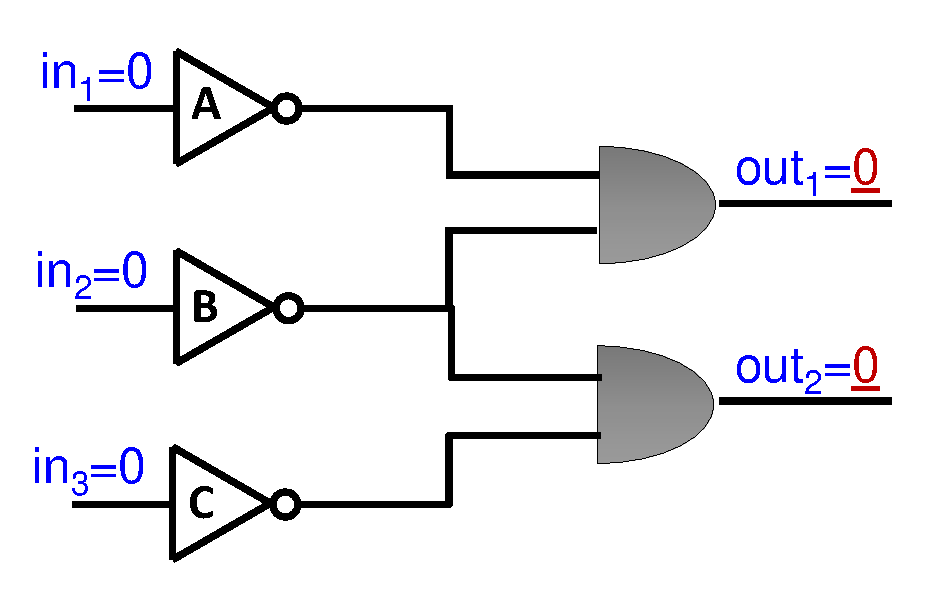
\includegraphics[width=0.5\columnwidth]{transition-example.pdf}%
\caption{An example to demonstrate the MDP transition functions used by \planbased .} %Assume that $p(\{B\})$=0.4, $p(\{B,A\})$=$p(\{B,C\})$=$p(\{A,C\})$=0.2. The possible system outputs after repairing $B$ would be $(0,0),(0,1),(1,0)$, $(1,1)$ with probability 0.2,0.2,0.2, and 0.4, respectively. The possible system outputs after repairing $A$ and $C$ would be $(0,0)$ and $(1,1)$ with probability 0.8 and 0.2, respectively.}
\vspace{-0.6cm}
\label{fig:transition-example}%
\end{center}
\end{figure}
%\end{wrapfigure}

% Example where several diagnoses have yield different observations
To demonstrate how the transition function is computed, consider the system described in Figure~\ref{fig:transition-example}. It is a logical circuit with outputs $(out_1,out_2)$ having an observed value of $(0,0)$ while the expected value is $(1,1)$. Assume that the diagnoses in $\Omega$ are $\{\{B\},\{B,A\},\{B,C\},\{A,C\}\}$, each with an abnormal behavior of flipping the value of its output, and the likelihoods of these diagnoses are 0.4, 0.2, 0.2, and 0.2, respectively\footnote{A diagnosis in $\Omega$ can be a subset of another diagnosis in $\Omega$.}. Consider the transition function for the possible outcomes of repairing $B$.
With 0.4 probability, the system is fixed.
With 0.2 probability, the correct diagnosis is $\{B,A\}$ and thus after fixing $\{B\}$ the system output would be $(0,1)$.
Similarly, there is a 0.2 probability to that the system output after repairing $\{B\}$ would be $(1,0)$ (for the case where the correct diagnosis is $\{B,C\}$),
and 0.2 probability for the system output to be $(0,0)$ (for the case where the correct diagnosis is $\{A,C\}$). Thus, repairing $B$ can lead to each of these 4 outcomes, and correspondingly to different MDP states.

% Example where several diagnoses have the same observations
Considering next the transition function for the possible outcomes of repairing $A$ and $C$. There is 0.2 probability that $\{A,C\}$ is the diagnosis, and subsets of $\{A,C\}$ are not diagnoses. Thus, there is a 0.2 probability for the system to be fixed. However, there is a 0.8 probability of observing $(0,0)$ after fixing $A$ and $C$, leading to the same MDP state for each of the remaining diagnoses  ($\{B\},\{B,A\},\{B,C\}$).


% What is a solution
A solution to an MDP is a policy, mapping every state to an action. In BRP, a policy maps every state reachable during the repair process to a repair action. We call such a policy a {\em repair policy}.

% Optimal solver
One can theoretically obtain an optimal repair policy by computing the optimal solution to the MDP above. There are several MDP solvers that return optimal solutions, such as value iteration, policy iteration~\cite{russell2010artificialIntelligence}, and LAO*~\cite{hansen2001lao}.
This would define the best repair action for every state reached during the repair process, where best means the repair action that minimizes the expected cost. We call this approach Optimal-BRP.

\subsection{State Space Size}
The state space of the MDP solved by Optimal-BRP is in practice too large to be solved optimally. First, the set of possible actions in a state is exponential in $|\overline{Repaired}|$, as every subset of $\overline{Repaired}$ can be a repair action. %[[Roni: footnote: can do operator decomposition to reduce branching factor at the cost of solution depth]]
Second, the number of states that can be reached after applying an action is also potentially exponential in the number of system outputs. This is because when a repair action fails, the set of possible observations is potentially equal to the number of diagnoses that are not ``fixed'' by the past repair actions. The number of such diagnoses can be exponential in the number of system components, but the number of different outputs is at most exponential in the number of system outputs.
%[[Add an example of both cases. Where the $\#diagnoses < 2^{\#outputs}$ and the other way around.]]
The state space described by our MDP is thus too large to be optimally solved in practice.
%$\meir{why dont you say that the action space is also exponential $2^{|COMPS|}$}[[Roni: I do.]]


However, solving MDPs with very large state spaces is a rapidly growing research field, especially when relaxing the requirement for optimal solutions. MDPs of a substantially larger scale can be solved suboptimally using an off-the-shelf suboptimal MDP solver. There are many suboptimal MDP solvers, such as Monte Carlo Planning (MCP)~\cite{silver2010monte} and Real-Time Dynamic Programming~\cite{barto1995learning}, as well as simply running Value or Policy iteration with earlier stopping conditions.
%%\section{BRP as a Combinatorial Optimization Problem}
\section{Myopic BRP}
\planbased\ computes a complete repair policy. Next, we describe a lighter-weight myopic approach, where only the next repair action is determined. We call this approach \myopic , and describe several ways to implement it.
\myopic\ searches the space of possible repair action, looking for the {\em best} repair action to perform next. The {\em best} repair action is defined with respect to a utility evaluation function $u(\cdot)$ that maps a repair action to a real value that estimates its merit.


% Myopic is still hard
Note the space of possible repair action is combinatorial, as it contains any subset of components from $\overline{Repaired}$. Thus, implementing \myopic\ requires defining $u(\cdot)$ and defining a search algorithm used to search for the best repair action.
The effectiveness of \myopic\ depends on the search algorithm and utility function used.
There are many existing heuristic search algorithm for searching large combinatorial search spaces~\cite{russell2010artificialIntelligence,edelkamp2011heuristic}. We therefore focus on proposing a set of possible utility functions that \myopic\ can use. Note that for some of the utility functions described next it is possible to find the best repair action without searching the entire $2^{\overline{Repaired}}$ search space.

\subsection{Best Diagnosis and Lowest Cost}
% MBDE to the rescue
A key source of information for all the utility functions described below is the set of diagnoses $\Omega$ and their likelihoods ($p(\cdot)$). These are obtained by using an MBDE over the observations of the current state of the system. We denote by {\em Best Diagnosis} (BD) and {\em Lowest Cost} (LC) two straightforward such utility functions.
BD returns a set of components that are assumed to be faulty in the most likely diagnosis. LC returns a set of components that are assumed faulty in a single diagnosis $\omega$ whose repair cost (cost(Repair($\omega$))) is minimal. BD and LC were proposed earlier in the context of software test planning~\cite{stern2012using,zamir2014using}. %[[Roni: I also cite our earlier DX paper, as it mentions LC while in our later paper we only mention BD. Maybe this is wrong.]]

Let $u_{BD}$ and $u_{LC}$ denote the utility functions used in \myopic\ for BD and LC respectively. Both $u_{BD}$ and $u_{LC}$ assign zero to sets of components that are not in $\Omega$. For $\omega\in \Omega$, $u_{BD}=p(\omega)$ and $u_{LC}=-cost(Repair(\omega^{-}))$.

%\meir{here and after when you say the heuristic is equal... it is somewhat confusing since people use to think about a heuristic as algorithm and here you refer it in terms of heuristic search as an estimation of an action cost. it should be clarified. Roni: no good idea how to do this}


% TODO: List limitations of BD and LC, although I think it is obvious.


\subsection{Minimizing Redundant Costs}
BD and LC are provided as baseline heuristics. Before describing the {\em expected cost} (EC) utility function we explain the over-arching reasoning behind it.
Repairing a system requires performing repair actions. An ideal utility function would assign zero to all repair actions except the repair action that is exactly the set of faulty components. As the set of faulty components is now known, an intelligent heuristic would cause \myopic\ to choose the repair action that minimizes the expected total repair cost.


Some repair costs are inevitable. These are the repair overhead of a single repair action, and the component repair costs that repair the faulty components. The EC utility function estimates the expected total repair costs beyond these inevitable costs. These are the costs incurred by repairing components that are not really faulty and the costs of the future repair actions required in case the current repair action does not fix the system. We refer to the first costs as the {\em false positives cost}, denoted by $cost_{FP}$, and to latter costs as {\em false negative cost}, denoted by $cost_{FN}$\footnote{Note that the term false negative is somewhat different here than how it is used in the Machine Learning literature.}.

Given $cost_{FP}$ and $cost_{FN}$ for a repair action $\gamma$ (denoted $cost_{FP}(\gamma)$ and $cost_{FN}(\gamma)$, respectively), the EC utility function, denoted $u_{EC}$, is computed as follows:
\[ cost_{FP}(\gamma)+(1-\sysrep{\gamma})\cdot cost_{FN}(\gamma)\]
%\meir{in the pdf it is not compiled well}
Note that $cost_{FN}(\gamma)$ is multiplied by $1-\sysrep{\gamma}$ as the false negatives costs are only incurred if the current repair action did not repair the system. As discussed above, the probability that this occurs is $\sysrep{\gamma}$. %[[Roni: maybe last sentence is redundant]]\meir{no, it is important}
\noindent Next, we discuss how to estimate $cost_{FP}$ and $cost_{FN}$.


\subsubsection{False Positives Cost}
The false positives cost can be computed by considering the {\em Component Fault Probabilities} (CFP)~\cite{stern2013findingAll}.
%\meir{we use here cfp rather than the new name. i think it is ok since that was the name in previous work. for a space problem we can shorten significantly this subsubsection}
%\begin{definition}[Component Fault Probability (CFP)]
%A CFP is a mapping $CFP:COMPS\rightarrow [0,1]$ intended to estimate the
%probability that a given component is faulty.
%\end{definition}
A CFP is a mapping $CFP:COMPS\rightarrow [0,1]$ that estimates the probability that a given component is faulty. 
Given $\Omega$ and $p$, a CFP can be generated by summing for every component $C$ the diagnosis likelihoods of diagnoses that $C$ is part of. 
%\noindent A CFP can be generated from $\Omega$ and $p$ as follows:
%\begin{equation}
%CFP(C)=\sum_{\omega\in\Omega}p(\omega)\cdot \mathbbm{1}_{C\in\omega}
%\label{eq:cfd}
%\end{equation}
%where $\mathbbm{1}_{C\in\omega}$ is the indicator function defined as:
%\[
%\mathbbm{1}_{C\in\omega}=
%\left\{
%\begin{array}{lr}
%	1 & C\in\omega \\
%	0 & \text{otherwise}
%\end{array}
%\right.
%\]
This way to generate CFP from $\Omega$ and $p$ was described in previous works~\cite{zamir2014using,feldman2013model,stern2013findingAll}. It is correct under the assumption that $p(\cdot)$ assigns correct and independent probabilities to the diagnoses in $\Omega$.

Given a CFP, the expected false positives cost of a repair action $\gamma$ can be computed as follows:
\[ cost_{FP}(\gamma)=\sum_{C_i\in \gamma} (1-CFP(C_i))\cdot cost(C_i) \]

%[[Roni: maybe say something about runtime ]]

\subsubsection{False Negatives Cost}
%$cost_{FN}$ requires estimating the number of future repair actions until the system is fixed. Thus, correctly estimating $cost_{FN}$ is more problematic than $cost_{FP}$, as it requires considering the future actions of the BRP solver (which is \myopic\ in this case).
Correctly estimating $cost_{FN}$ is more problematic than $cost_{FP}$, as it requires considering the future actions of the BRP solver (which is \myopic\ in this case). 
%\meir{here is the place to add a sentence which explains why it should consider future actions.Roni:added above, hope it is good}
In the best case, only one additional repair action would be needed. In the worst case, there would be a single repair action for every component that was not repaired. Thus, an estimate of $cost_{FN}$ should be a value in the range $[cost_{repair},cost_{repair}\cdot |\overline{Repaired}|]$.
%\meir{i do not remember you defined $C_{repair}$ Roni: my mistake. changed to cost_{Repair}
One can estimate $cost_{FN}$ by choosing a random number in this range.

%[[Roni: maybe add here some more thoughtful ideas on how to estimate]]


%The key problem in estimating $cost_{FN}$ is that it depends on the future choices done by \myopic\, which in turn depends on how $cost_{FN}$ is estimated (if using $u_{EC}$). 
To fully consider the future costs of the repair process, one needs to {\em plan} them ahead. The \planbased\ does this explicitly at the cost of incurring substantially more computational efforts.
%\section{Optimal Batch Repair Planner}
Following the maximum expected utility principle, we consider a decision making process for BRP as optimal if it minimizes the expected repair costs. To solve BRP optimally we model it as a stochastic shortest path Markov Decision Process (MDP). \meir{nnot all readers are well familiar with mdp and its utilized. i propose that here you say what mdp knows to solve and why we think it is compatible to our problem.}

Such an MDP is defined by a tuple $\langle S,A,Tr,R,I,G \rangle$, where $S$ and $A$ are the sets of states and actions as described in the previous section. $Tr(s,a,s?)$ is the transition function, computing the probability that performing an action $a$ at state $s$ would lead to a state $s?$. $R(s,a)$ is the reward of performing an action $a$ at state $s$. $I$ is the initial states and $G$ is the set of terminal states.

In our case, states and actions are as defined above: states are the observed behavior of the system and the set of components repaired so far, and an action is a repair action (applied to a set of components). The reward of performing an action is minus the cost of the corresponding repair action. The possible outcomes of an action is either that the system is repaired or it is not. The probability of each outcome is dictated by {\tt SysRepair()}. The repaired system outcome corresponds to a goal state.\meir{maybe here is the place to move the last sentence of the next para where you define the goal state.}

%If the system is not repaired, then a new state is reached, according to the new observation, obtained when testing the system after performing the last repair action.
Consider the other outcome, where the system is not repairs. In such a case, the system would be tested, resulting in a new observation. What will be this new observation depends on the true diagnosis \meir{I think you used the term "correct diagnosis", no?}. Thus, the set of diagnoses returned by the MBDE allows computing the possible new observations, and the diagnosis likelihoods gives the transition probabilities. A state is a goal state if it represents a state where the system is repaired, i.e., when the last observation is that all outputs yield their nominal output. [[Roni: not the best phrasing]]\meir{the transition function is not explained well at all. an example may help}

% What is a solution
A solution to an MDP is a policy, mapping every state to an action. In BRP, a policy maps every state reachable during the repair process to a repair action. We call such a policy a {\em repair policy}.

% Optimal solver
One can theoretically obtain an optimal repair policy by computing the optimal solution to the MDP above. This would define the best repair action for every state reached during the repair process, where best means the repair action that minimizes the expected cost. We call this approach Optimal-BRP.\meir{dont you call it \planbased\ ?}

\subsection{State Space Size}
The state space of the MDP solved by Optimal-BRP is in practice too large to be solved optimally. First, the set of possible actions in every state is in the worst case $2^{|COMPS|}$, as every subset of components may be fixed. [[Roni: footnote: can do operator decomposition to reduce branching factor at the cost of solution depth]]

Second, the number of states that can be reached after applying an action is also potentially exponential in the number of system outputs. This is because when a repair action fails, the set of possible observations is potentially equal to the number of diagnoses that are not ``fixed'' by the past repair actions. The number of such diagnoses can be exponential in the number of system components, but the number of different outputs is at most exponential in the number of system outputs.
[[Add an example of both cases. Where the $\#diagnoses < 2^{\#outputs}$ and the other way around.]]
The state space described by our MDP is thus too large to be optimally solved in practice.
\meir{why dont you say that the action space is also exponential $2^{|COMPS|}$}
%\section{Diagnoses and Possible Repair Actions}
In both \myopic\ and \planbased\ algorithms, the possible repair actions considered at a system state is to be $2^{\overline{Repaired}}$. This indeed covers all relevant repair actions, but results in a high computationally complexity. For \myopic\ this is the size of the search space and in \planbased\ this is the branching factor of the corresponding MDP state space.
Thus, one way to speedup \myopic\ and \planbased\ is to relax the requirement to consider all $2^{\overline{Repaired}}$ repair actions. This can result in faster runtime at the potential cost of finding solutions of lower quality.

\subsection{Helpful Repair Actions}
% Can be optimal even if only considering just the components in the diagnoes
The first relaxation we propose is called {\em Helpful Repair Actions} (HRA). It is a straightforward relaxation that still results in \planbased\ outputting an optimal repair policy if $\Omega$ contains all diagnoses.
%\meir{must we assume p is correct? dont we assume this along all the paper? if we assume this then such a comment makes the reader some confused, since it will look for the implications of such an assumption.}{Roni: you're right, we dont need this assumption. Fixed it}
In such a case, components that are not part of any diagnoses cannot be faulty. Thus, instead of considering to repair every component in $\overline{Repaired}$, a BRP solver can consider to repair only components that are part of at least one diagnosis. The set of such components is denoted by $\overline{Repaired}[\Omega]$. Formally,
\[ \overline{Repaired}[\Omega]=\{C|C\in \overline{Repaired}\ \wedge \exists \omega\in \Omega\ \text{s.t.}\ C\in\omega \}\]

% Even if not optimal, it's stil reasonable
Restricting the applicable repair actions to return only subsets of $\overline{Repaired}[\Omega]$ is also reasonable when $\Omega$ does not return all diagnoses, under the assumption that the diagnoses found in $\Omega$ are more informed than random guesses. In such cases, however, \planbased\ cannot guarantee to find the optimal repair plan.


% Consider only supersets of diagnoses
\subsection{Must Fix Repair Actions}
The {\em Must Fix Repair Actions} (MFRA) relaxation further restricts the set of repair actions to only those that may immediately fix the system. If $\Omega$ contains all diagnoses, then to fix the system a repair action must repair at least all the components of one of the diagnoses in $\Omega$. Thus, the set of repair actions considered by MFRA is all the subsets of $\overline{Repaired}[\Omega]$ such that there exists a diagnosis in $\Omega$ whose faulty components are repaired. This set is denoted by $MFRA[\Omega]$. $MFRA[\Omega]$ is defined below more formally.
\[ MFRA[\Omega]=\{ \gamma | \gamma\subseteq \overline{Repaired}[\Omega] \wedge \exists \omega\in\Omega \text{ s.t. } \omega^{-}\in\gamma\}\]
The motivation behind MFRA is to reduce future repair overheads -- avoiding repair actions that we know would not fix the system.

% When to use
MFRA would be suitable especially to cases where the repair overhead is much more costly than the component repair costs ($cost_{repair}>>cost_{C_i}$).
If the component repair costs are not substantially less than the repair overhead, then MFRA may not be a good solution, as it might be useful to perform a repair action just to obtain another observation, resulting in a more accurate diagnoses that may save component repair costs.



\subsection{Relaxing the MBDE}
% MBDE was assumed to return all diagnoses % Returning all diagnosis is hard, there may be many of those
All the algorithms, heuristics and relaxations, so far assumed, either implicitly or explicitly, that $\Omega$ contains all diagnoses. This is especially important to the correctness of how the transition function in the \planbased\ MDP was defined, and the MFRA relaxation presented above. Finding all diagnoses, however, is a very hard task computationally~\cite{Selman90}. Moreover, considering all diagnoses as possible repair actions is likely to be too computationally expensive for \myopic\ and \planbased . As an alternative, diagnosis algorithms such as Sherlock~\cite{deKleer1989diagnosis} and CDA*~\cite{williams2007conflict} return the most likely diagnoses. Under some assumptions, these are the diagnoses with the smallest number of abnormal components (also known as the minimal cardinality diagnoses), and much work has been done on finding such diagnoses~\cite{metodi2012compiling,stern2012exploring,de2011hitting,de1987diagnosing}.


% Minimal cardinality and all kernels
%Others return the diagnoses with the smallest number of abnormal components (also known as the minimal cardinality diagnoses), which under some assumptions translate to the most likely diagnoses~\cite{metodi2012compiling,stern2012exploring,de2011hitting,de1987diagnosing}. Another option is to return all kernel diagnoses, which according to Equation~\ref{eq:likelihoods} are more likely than the diagnoses they cover. Note that in weak fault models, which is where the system description ($SD$) only contains the nominal behavior of the components, kernel diagnoses are in fact {\em subset minimal diagnoses}. A diagnosis $\omega$ is subset minimal if there is no diagnosis $\omega'$ such that $\omega'^{-}\subset\omega^{-}$. Searching for subset minimal diagnoses in weak fault models is a well-studied problem in the model-based diagnosis literature~\cite{de1987diagnosing}.


% SAFARI
%The set of kernel diagnoses can, however, be very large and finding kernel diagnoses is computationally hard~\cite{deKleer1990characterizing}. More generally, finding the most likely diagnoses may not be feasible in reasonable time. Thus, approximate diagnosis algorithms may be required. For example, the SAFARI algorithm performs a local search until a diagnosis is found, and then tries to minimize it stochastically~\cite{feldman2010approximate}.\meir{as you know it is only for WFM. but you have already mentioned CDA* which computes only the most probable diagnoses.s}

% Why most likely is not a horrible choice
Implementing MBDE so as to not return all diagnoses, e.g., using one of the algorithms specified above, may affect the performance of \myopic\ and \planbased\ .
Below, we give a partial list of the effects of having $\Omega$ not contains all diagnoses.\\
%\begin{itemize}
	\noindent {\bf Partial repair actions.} Both HRA or MFRA limit the set of repair actions applicable according to a given set of diagnoses. If, for example, a faulty component $C_i$ does not occur in any diagnosis, then repairing it would not be a repair action considered by either \myopic\ or \planbased\footnote{Note that if MBDE is guaranteed to always find at least one diagnoses until the system is fixed, then \myopic\ and \planbased\ would also eventually fix the system.}.\\
	\noindent {\bf Inaccurate diagnoses likelihoods.} The diagnoses likelihoods computed according to Equation~\ref{eq:likelihoods}, where the denominator normalizes the diagnosis likelihood of a single diagnosis with that of all the diagnoses. With a limited set of diagnoses, the likelihoods computed by Equation~\ref{eq:likelihoods} would be higher than their true value. This would affect the accuracy of {\tt SystemRepair}, CFP and the MDP transition function.	
%\end{itemize}
%The impact of not returning the set of all diagnoses depends on the likelihood of the diagnoses that are returned. Let $\Omega_b$ denote the set of diagnoses returned by an MBDE, and let $\Omega^*$ denote the set of all diagnoses. Returning $\Omega_b$ instead of $\Omega^*$ has two affects. First, the set of repair actions may be limited, if either HRA or MFRA are used. Second, the diagnoses likelihoods become less accurate, as the denominator of Equation~\ref{eq:likelihoods} would not be based on $\Omega^*$. The accuracy of the diagnoses likelihoods affects the accuracy of \sysrep , the CFP, and the transition function of \planbased .
%\meir{for space limitation we can delete the next.}
%The negative effects of not returning all the diagnoses are controlled by the probability mass of the likelihoods of the returned diagnoses. Intuitively, if the most likely diagnoses are substantially more likely than the less likely diagnoses, then the missed repair action would probably not be repair actions worth executing and the inaccuracies in the computed diagnoses likelihoods would be potentially smaller. Studying the exact impact is left for future work.

%\meir{the subsubsection is too long and mess. the last para is really the most important and we need only one para beforehand that says that there are alternatives to finding all diagnoses such as SHERLOCK \cite{deKleer1992} and CDA*.} [[Roni: repharased]]



\section{BRP as a Combinatorial Search}
As mentioned in the introduction, the approach for solving BRP that we pursue in this paper formulates BRP as a combinatorial search problem. The search space is the space of possible repair actions, i.e., every subset of the set of components there were not repaired yet.
The search problem is to find the repair action that maximizes a utility evaluation function $u(\cdot)$ that maps a repair action to a real value that estimates its merit.


% Myopic is still hard
%Implementing this search-based approach for BRP requires defining $u(\cdot)$ and defining a search algorithm used to search for the best repair action.
The effectiveness of this search-based approach for BRP depends on the search algorithm used and how the $u(\cdot)$ utility function is defined.
There are many existing heuristic search algorithm for searching large combinatorial search spaces~\cite{russell2010artificialIntelligence,edelkamp2011heuristic}. Thus, in this work we propose and evaluate a set of possible utility functions. Note that for some of the utility functions described next it is possible to find the best repair action without searching the entire search space of possible actions, while others are more computationally intensive.


\subsection{$k$ Highest Probability}

A key source of information for all the utility functions described below is the set of diagnoses $\Omega$ and their likelihoods ($p(\cdot)$). We assume that this information is obtained by using a diagnosis engine over the observations of the current state of the system. The set of returned diagnoses may be very large. The first utility function we propose is based on the system's {\em health state}, which has been recently proposed as a method for aggregating information from a set of diagnoses~\cite{Stern15shely}.

\begin{definition}[Health State]
A health state is a mapping $F: COMPS\rightarrow [0,1]$ where
\[ \displaystyle F(C)=\sum_{\omega\in \Omega s.t. C\in \omega} p(\omega)\]
\label{def:health-state}
\end{definition}
$F(C)$ is an estimate of the likelihood that component $C$ is faulty given a set of diagnoses $\Omega$ and their likelihoods.
Based on the system's health state, we propose the following utility function, denoted $u_{HP}$:
\[
u_{HP}(\gamma) = \sum_{C\in \gamma} F(C)
\]
where $\gamma$ is a subset of $COMPS$ that were not repaired yet.


The repair action that maximizes $u_{HP}$ is trivial --- repair all components.
This would result in the system being repairs, but of course, may repair many components that are likely to be healthy. To mitigate this effect, we propose the {\em $k$ highest probability} repair algorithm ($k$-HP), which limits the number of components that can be repaired in a single repair action to $k$, where $k$ is a user-defined parameter. Note that computing $k$-HP does not need any exhaustive search: simply sort the health state in descending order of $F(\cdot)$ values and repair the first $k$ components.


The $k$-HP repair algorithm has two clear disadvantages. First, the user needs to define $k$. Second, $k$-HP does not consider repair costs (neither component repair costs nor overhead costs).
%MEIR: i did not understand the last sentence.
The next set of utility functions and corresponding repair algorithms address these disadvantages.



\subsection{Wasted Costs Utilities}

%Before describing the next set of proposed utility functions we explain the over-arching reasoning behind it.
Repairing a system requires performing repair actions. %An ideal utility function would assign zero to all repair actions except the repair action that is exactly the set of faulty components, and the corresponding repair algorithm would then choose a single batch repair action that repairs these components.
Some repair costs are inevitable. These are the repair overhead of a single repair action, and the component repair costs that repair the faulty components. We propose a family of utility functions that try to estimate the expected total repair costs beyond these inevitable costs. We refer to these costs as {\em wasted costs} and to utility functions of this family as {\em wasted cost functions}. We model these wasted costs as being composed of two parts.
\begin{itemize}
\item {\bf False positive costs ($cost_{FP}$).} These are the costs incurred by repairing components that are not really faulty.
\item {\bf False negative costs ($cost_{FN}$).} These are the overhead costs incurred by future repair actions.
\end{itemize}
It is clear why the false positive costs are wasted costs --- these are repair costs incurred on repairing healthy components. The false negative costs are wasted costs because if one knew upfront which components are faulty, then the optimal repair algorithm would repair all these components in a single batch repair action, incurring no further overhead costs. Thus, future overhead costs represent wasted costs.


We borrow the terminology of false positive and false negative from the machine learning literature, but use it in a somewhat different manner. To explain this choice of terminology, assume that positive and negative mean faulty and healthy components respectively. Choosing to repair a faulty component is regarded as a true positive, and not repairing a healthy component is regarded as a true negative. Thus, the wasted costs incurred by repairing healthy components are costs incurred due to false positives, and the wasted costs incurred by not repairing a faulty component are overhead costs incurred due to false negatives. While this is not a perfect match in terminology, we belief that it helps clarify the underlying intention of $cost_{FP}$ and $cost_{FN}$.


\subsubsection{The Wasted Cost Utility Function}
For a given set of components $\gamma$, we denote by $cost_{FP}(\gamma)$ and $cost_{FN}(\gamma)$ the false positive costs and false negative costs, respectively, incurred by performing a batch repair action of repairing all the components in $\gamma$. Given $cost_{FP}(\gamma)$ and $cost_{FN}(\gamma)$, we propose the following general formula for computing the expected wasted costs, denoted by $C_{WC}$.
\[ C_{WC}=cost_{FP}(\gamma)+(1-\sysrep{\gamma})\cdot cost_{FN}(\gamma)\]
%\meir{in the pdf it is not compiled well}
The left hand side of the formula is the false positive costs. The right hand side of the formula is the false negative costs, multiplied by the probability that the system will not be fixed by repairing the components in $\gamma$. Thus, the formula gives the total expected wasted costs.
We define $U_{WC}=-C_{WC}$ as the {\em wasted cost utility function}.



The wasted cost utility function is a theoretical utility function, since one does not know upfront the values of $cost_{FP}$ and $cost_{FN}$. Next, we propose several ways to estimate $U_{WC}$ by proposing ways to estimate $cost_{FP}$ and $cost_{FN}$.

%[[Roni: maybe last sentence is redundant]]\meir{no, it is important}
%\noindent Next, we discuss how to estimate $cost_{FP}$ and $cost_{FN}$.

\subsubsection{Estimating the False Positives Cost:}
We propose to estimate the false positive costs by considering the system's health state (Definition~\ref{def:health-state}), as follows.

\[ \widehat{cost}_{FP}(\gamma)=\sum_{C\in \gamma} (1-F(C))\cdot cost(C) \]
This estimate of the false positive costs can be understood as an expectation over the false positive costs. The cost of a repaired component $C\in\gamma$ is part of the false positive costs only if $C$ is in fact healthy. The probability of this occurring is $(1-F(C))$. Thus, $(1-F(C))\cdot cost(C)$ is the expected false positive cost due to repairing component $C$.



\subsubsection{Estimating the False Negatives Cost:}
Correctly estimating $cost_{FN}$ is more problematic than $cost_{FP}$, as it requires considering the future actions of the repair algorithm.
In the best case, only one additional repair action would be needed. This would incur a single additional overhead cost. We call this {\bf the optimistic $cost_{FN}$}, or simply $cost_{FN}^o$, which is equal to $cost_{repair}$.
The other extreme assumes that every component not repaired so far would be repaired by a single repair action, and correspondingly an incurred overhead cost. We experimented with a slightly less extreme estimate, in which we assume that only faulty components will be repaired in the future, but each will be repaired in a single repair action, incurring one $cost_{repair}$ per faulty component.
Since we do not know the number of faulty components, we use the expected number of faulty components according to the health state: $\sum_{c\notin \gamma} F(c)$. The resulting estimate is referred to as {\bf the pessimistic $cost_{FN}$}, denoted by $cost_{FN}^p$, is thus computed as:
\[ cost_{FN}^p(\gamma)=cost_{repair}\cdot \sum_{c\notin \gamma} F(c)\]

%relax the computation done in each component so that a possible suboptimal but feasible solution is obtained.

To summarize, we propose two utility functions from the wasted cost utility function family. A pessimistic wasted cost function, that uses $\widehat{cost}_{FP}$ and $cost_{FN}^p$ to estimate $cost_{FP}$ and $cost_{FN}$, and an optimistic wasted cost function that uses $\widehat{cost}_{FP}$ and $cost_{FN}^o$. The corresponding repair algorithms search in the combinatorial space of all possible sets of components to find the set of components that maximizes $U_{WC}$.

%The repair action used to compute

\subsection{Handling the Computational Complexity}
The search space is very large --- the size of the power set of all components that were not repaired so far.
We explored two simple ways to handle this. The first approach is to only consider subset of components with up to $k$ components, where $k$ is a parameter. We set the components in a decreasing order of their health state (Definition \ref{def:health-state}) and choose the first $k$ components. Thus we increase the probability of repairing faulty components. This approach is referred to as {\bf Powerset-based search}.

The second approach considers only supersets of the diagnoses in $\Omega$. This has the intuitive reasoning that at least one of these diagnoses is supposed to be true (according to the known observation), and thus a repair algorithm should try to aim for fixing the problem in the next repair action. Thus, in this approach, we considered in the search for the best repair action every set of components that are unions of at most $k$ diagnoses, where $k$ is a parameter. We set the diagnoses in a decreasing order of their likelihood (Equation \ref{eq:likelihoods}) and choose the first $k$ diagnoses. Thus we increase the probability of repairing faulty components. This approach is referred to as the {\bf Union-based search}. %Experimentally, the union-based search approach yielded much better results than the powerset-based search and thus we only show results for it in the experimental results below.

For both powerset-based search and union-based search, increasing $k$ results in a larger search space and consequently higher computational complexity. On the other hand, a large search space increases the range of repair actions considered, and thus higher $k$ can potentially find better repair actions. This provides an often desired tradeoff of computation vs. solution quality. This trend is observable in our experimental results below.


\section{Experimental Results}

We evaluated the proposed batch selection algorithms on standard Boolean circuit systems. Figure \ref{fig:74181} presents a logic diagram of one of these systems, a known MSI chip called the 74181. It is an arithmetic logic unit (ALU) that provides thirty-two functions of two 4-bit variables. $\COMPS$ in this example include the Boolean gates in the ALU. $\SD$ is the behavior description of the components, for instance, the healthy behavior of an $\textit{OR}$ gate implies the ``$\textit{OR}$'' behavior while abnormal behaviors can be stuck at 1 or at 0. $\OBS$ includes the inputs and outputs of the ALU. A diagnosis states which gates are healthy and which are in a faulty mode. The batch repair algorithms propose a set of gates to fix.

\begin{table}\centering
{\small
\begin{tabular}{|l|r|r|r|r|}
\hline
 {\bf Name} & {\bf $|${\tiny \COMPS}$|$} & {\bf in} & {\bf out} & {\bf \#observations} \\
\hline
    74181  & 65    & 14   & 8    & 26 \\
    74182  & 19    & 9    & 5    & 25 \\
    74283  & 36    & 9    & 5    & 22 \\
\hline
    c432   & 160   & 36   & 7    & 23\\
    c499   & 202   & 41   & 32   & 22\\
    c880   & 383   & 60   & 26   &  30\\
\hline
\end{tabular}
\caption{The Benchmark suite: systems  {\small 74XXX} and
         {\small ISCAS-85}, and scenarios Feldman.}
\label{tab:systems}
}
\end{table}%

The standard Boolean circuits we used in our experiments are presented in Table \ref{tab:systems}. The systems {\small 74XXX}~\cite{Hansen99} are described in the first three rows, and additional three systems of {\small ISCAS-85} \cite{Brglez89} are described in the following three rows. Observations were selected randomly from Feldman et al.'s~\shortcite{feldman2010approximate} known benchmark.
To adapt these benchmark systems and observations to be an experimental infrastructure for batch repair algorithms we set the prior probability of each gate to be faulty to 0.01 and chose a single diagnosis for each observation to serve as the injected faults. This is needed to decide when the system is fixed. Note that this ``true'' diagnosis was chosen with probability proportional to its likelihood of being correct, computed according to the priors mentioned above under the standard assumption of fault independence. The component repair cost was set to 5, and we experimented with repair overhead ($cost_{repair}$) costs of 10, 15, 20, and 25.

All batch repair algorithms used a simple MBDE based on exhaustive search to generate diagnoses. Diagnoses were generated in order of increasing cardinality, and halted after either all subset minimal diagnoses were found or a timeout of 15 minutes was reached. We did not use a more sophisticated MBDE as it is not the focus of this work. Note that the batch repair algorithms are applicable to any MBDE.


%We run the batch repair algorithms with different instances of fault injection on standard Boolean circuits presented in Table \ref{tab:systems}. The systems {\small 74XXX}~\cite{Hansen99} are described in the first three rows, and additional three systems of {\small ISCAS-85} \cite{Brglez89} are described in the following three rows. To adapt the Boolean circuits as an experimental infrastructure for batch repair algorithms we set the prior probability of each gate to be faulty to 0.01 and its repair cost to 5. Then, observations were selected randomly from Feldman et al.'s~\shortcite{feldman2010approximate} known benchmark, and a single diagnosis of these observations were selected as the true faults. A diagnosis was selected as the true fault with probability proportional to its likelihood of being correct, computed according to the priors mentioned above under the standard assumption of fault independence. Given an observation, all subset minimal diagnoses were found using exhaustive search. Note that the batch repair methods are indifferent to the diagnosis algorithms.  Also, we experimented with repair overhead ($cost_{repair}$) costs of 10, 15, 20, and 25.

%. An observation was generated by injecting faults to some gates and computing the outputs by propagating random inputs. We varied the number of injected faults in a range of 1--4.
%For lack of space we do not add details about the diagnosis algorithm since the main novelty of this paper is by proposing batch repair methods.

\begin{figure}{}%{4cm}
\begin{center}
  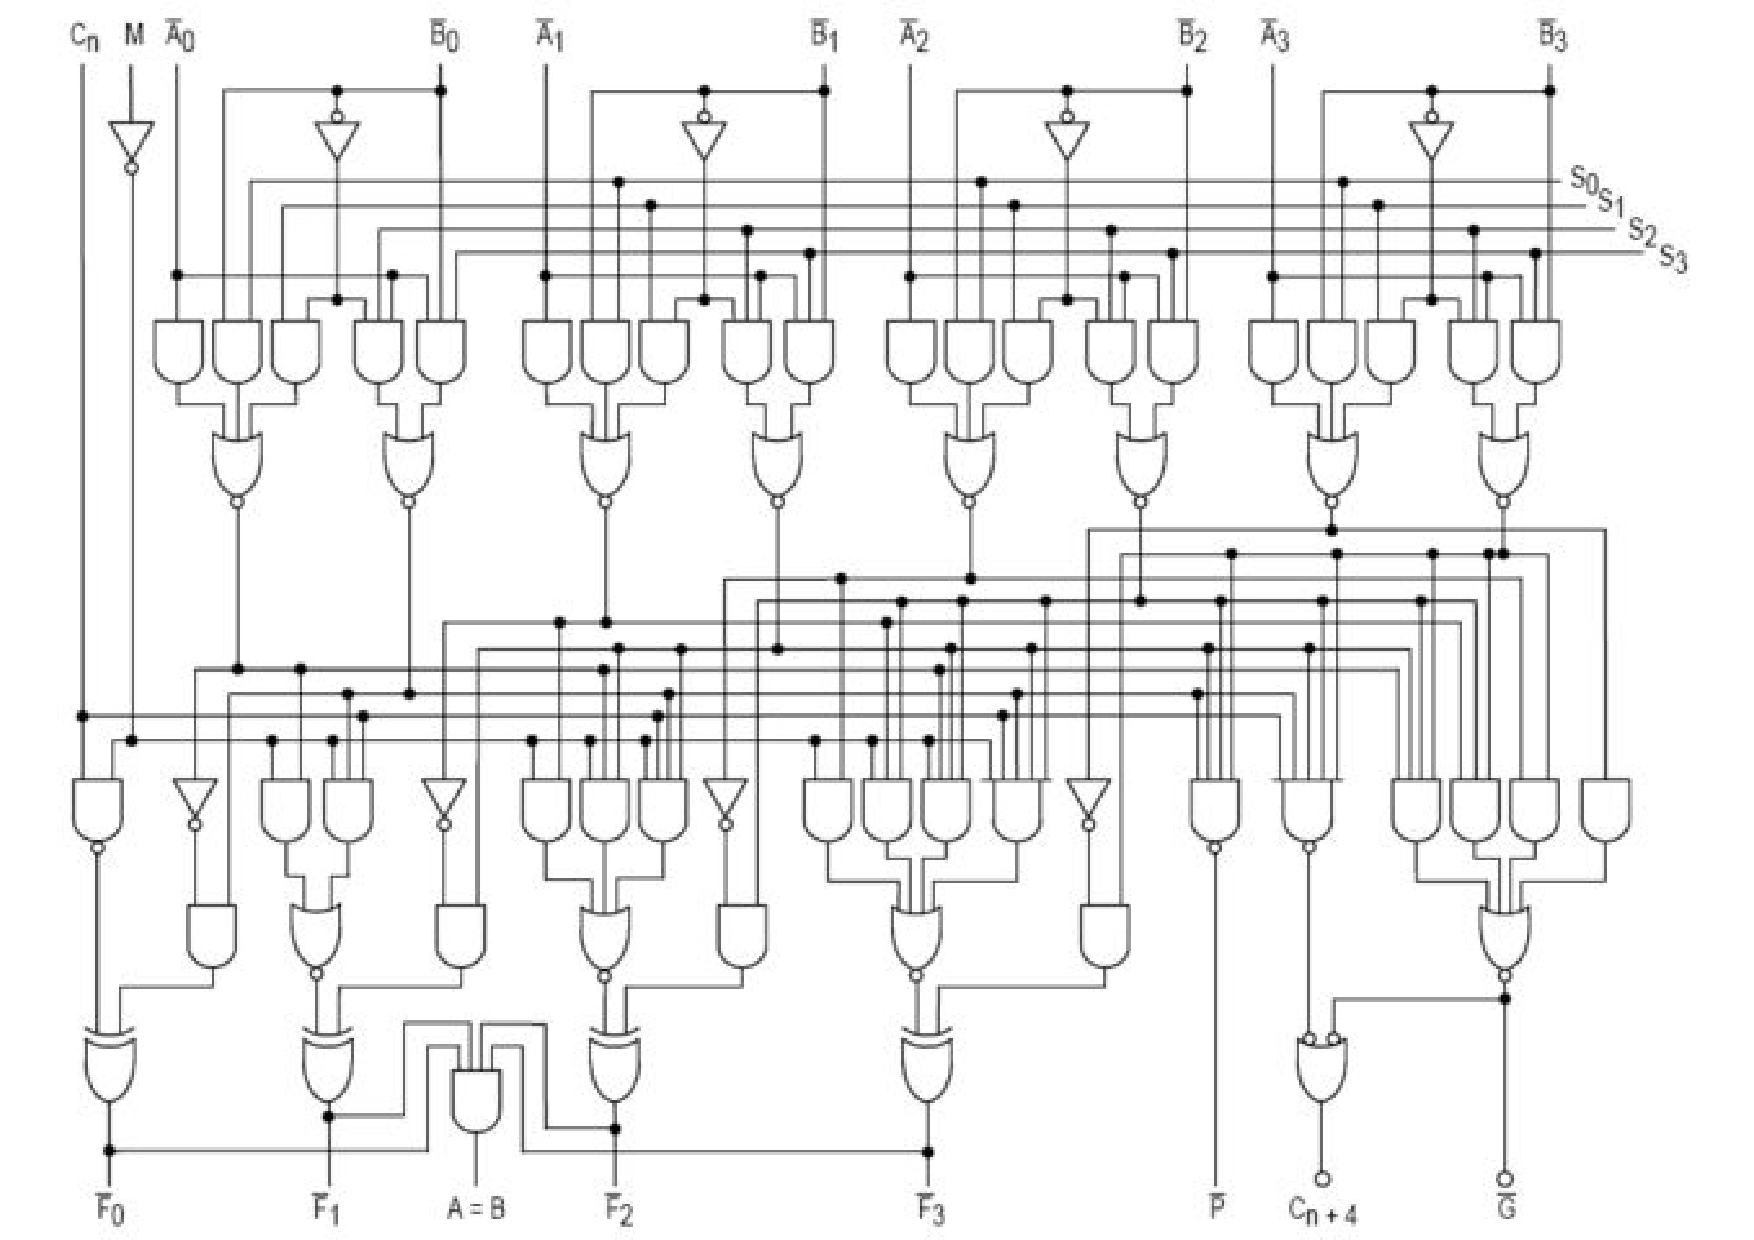
\includegraphics[width=0.9\columnwidth]{figures/74181.pdf}
  \caption{A logic diagram of ALU 74181.}
  \label{fig:74181}
\end{center}
\end{figure}


\subsection{Baseline Repair Algorithms}
%The main hypothesis of this line of work is that performing a batch repair action can save repair costs. To evaluate if the proposed batch repair algorithms are able to do so, we compare them with two repair algorithms that do not consider batch repair actions. These baseline repair algorithms, named ``Best Diagnosis'' (BD) and ``Highest Probability'' (HP),  are inspired by previous work on test planning~\cite{zamir2014using} and work as follows. BD chooses to repair a single component from the most preferred diagnosis in $\Omega$ (that with the highest $p(\cdot)$ value). From the set of components in the most probable diagnosis, BD chooses to repair the one with the lowest repair costs. The HP repair algorithm chooses to repair the component that is most likely to be faulty, as computed by the system's health state ($F[\cdot]$).

The main hypothesis of this line of work is that performing a batch repair action can save repair costs. To evaluate if the proposed batch repair algorithms are able to do so we compare them with 1-HP, in which the component that is most likely to be faulty is repaired. A similar approach was used by previous work on test planning~\cite{zamir2014using}. Another baseline repair algorithm we evaluated experimentally is to repair all components of the most likely diagnosis in a single batch repair action denoted {\em Batch Best Diagnosis} (hereinafter, BD-batch).

%.\meir{I think that the next comment is confusing and adds nothing} Note that this algorithm, denoted {\em Batch Best Diagnosis}, ignores repair costs, and serves as an extreme alternative to the BD algorithm that repairs a single component from the most likely diagnosis.



\subsection{Results}

\begin{table*}[htb]
\centering
\scriptsize
%\begin{tabular}{@{}lp{0.05cm}p{0.05cm}p{0.05cm}p{0.05cm}|rrrr|rrrr|rrrr|rrrr|rrrr@{}}
%\begin{tabular}{@{}lp{0.2cm}p{0.2cm}p{0.2cm}p{0.2cm}p{0.2cm}p{0.2cm}p{0.2cm}p{0.2cm}p{0.2cm}p{0.2cm}p{0.2cm}p{0.2cm}p{0.2cm}p{0.2cm}p{0.2cm}p{0.2cm}p{0.2cm}p{0.2cm}p{0.2cm}p{0.2cm}p{0.2cm}p{0.2cm}p{0.2cm}p{0.2m}@{}}
\setlength{\tabcolsep}{5pt}
\resizebox{\textwidth}{!}{
\begin{tabular}{l|rrrr|rrrr|rrrr|rrrr|rrrr|rrrr}
\hline
System   & \multicolumn{4}{c|}{74182}                 & \multicolumn{4}{c|}{74283}                 & \multicolumn{4}{c|}{74181}                   & \multicolumn{4}{c|}{c432}                  & \multicolumn{4}{c|}{c499}                  & \multicolumn{4}{c}{c880}                     \\ \hline
Overhead & 10       & 15       & 20       & 25       & 10       & 15       & 20       & 25       & 10       & 15       & 20        & 25        & 10       & 15       & 20       & 25       & 10       & 15       & 20       & 25       & 10       & 15        & 20        & 25        \\ \hline
1-HP     & 82       & 110      & 137      & 164      & 106      & 142      & 177      & 213      & 119      & 159      & 199       & 239       & 60    & 80    & 100   & 120   & 41    & 55       & 69       & 83       & 144      & 191       & 239       & 287       \\
BD       & 59       & 73       & 88       & 103      & 81       & 101      & 122      & 142      & 92       & 115      & 137       & 160       & 83       & 109      & 135      & 161      & {\bf 28} & 36       & 45       & 53       & 95       & 123       & 151       & 178       \\
2-HP     & 62       & 78       & 94       & 109      & 85       & 107      & 128      & 149      & 85       & 107      & 128       & 149       & 47       & 59       & 71       & 83       & 32       & 40       & 49       & 51       & 90       & 109       & 127       & 145       \\
3-HP     & 57       & 69       & 81       & 93       & 77       & 93       & 108      & 124      & 83       & 99       & 116       & 132       & {\bf 44} & {\bf 53} & {\bf 62} & 72       & 30       & 37       & 44       & 46       & {\bf 87} & {\bf 102} & {\bf 117} & {\bf 131} \\
4-HP     & 58       & 69       & 79       & 90       & 78       & 91       & 104      & 117      & 82       & 96       & 110       & 124       & 47       & 55       & 63       & 72       & {\bf 28} & {\bf 34} & {\bf 40} & 62       & 117      & 151       & 186       & 220       \\
Opt. (1) & 56       & 69       & 83       & 97       & 70       & 89       & 108      & 125      & 76       & 95       & 113       & 131       & 50       & 65       & 79       & 94       & 33       & 43       & 52       & 62       & 117      & 151       & 186       & 220       \\
Opt. (2) & {\bf 54} & 65       & 71       & 82       & 68       & 82       & 95       & 103      & {\bf 75} & 91       & 107       & 121       & 51       & 63       & 73       & 84       & 33       & 41       & 49       & 52       & 114      & 147       & 179       & 207       \\
Pes. (1) & 58       & 69       & 81       & 97       & 68       & 89       & 109      & 128      & 77       & 95       & 111       & 129       & 51       & 65       & 76       & 88       & 33       & 43       & 52       & 62       & 118      & 153       & 187       & 225       \\
Pes. (2) & 56       & {\bf 58} & {\bf 64} & {\bf 73} & {\bf 65} & {\bf 73} & {\bf 83} & {\bf 91} & 76       & {\bf 90} & {\bf 102} & {\bf 110} & 51       & 61       & 63       & {\bf 69} & 32       & 40       & 45       & {\bf 49} & 118      & 149       & 178       & 205      \\ \hline
\end{tabular}
}
\caption{Average repair costs until system is fixed.}
\label{tab:cost-results}
\end{table*}



Table~\ref{tab:cost-results} shows the average repair costs incurred until the system was fixed for the systems and problem instances described above.
The first column lists the name of the compared algorithms, where $Opt.(\cdot)$ and $Pes.(\cdot)$ denote the union-based search using either pessimistic or the optimistic wasted costs utility functions, i.e., where
 $cost_{FN}^p$ and $cost_{FN}^o$ are used to estimate $cost_{FN}$, respectively, and the number in brackets (either 1 or 2) is the value of $k$. We did not experiment with larger values of $k$ due to computational complexity. 
The powerset-based search approach yielded substantially worse results compared to the union-based results so we do not display it in Table~\ref{tab:cost-results}.
The other columns in Table~\ref{tab:cost-results} show the results for different overhead costs -- 10, 15,20, and 25. For every system and column, we marked in bold the best performing algorithm for every combination of repair overhead cost and system.

%In our experiments these were the $k$-HP repair algorithm for $k=4$ and the union-based search repair algorithm for $k=2$ using either the pessimistic or the optimistic wasted costs utility functions (i.e., where  $cost_{FN}^p$ and $cost_{FN}^o$ are used to estimate $cost_{FN}$, respectively). These algorithms are marked in Table~\ref{tab:cost-results} by ``4-HP'', ``Pes. (2)'', and ``Opt. (2)''. We observed in both types of algorithms -- $k-HP$, $Pes. (k)$, and $Opt. (k)$ -- that increasing $k$ resulted in higher runtime and usually better results, but we  could not run larger values of $k$ in reasonable time.


The first trend we highlight is that in all cases, using a batch repair algorithm resulted in significantly less costs compared to the 1-HP, in which a single component is repaired in each round. This supports our main claim that reasoning about the possibility of batch repair is important. For example, in the 74181 system when the repair overhead is 25, 1-HP required an average cost of 239 while Pes.(2) needed only 110.  


Increasing the repair overhead causes all algorithms to require more cost to fix the system. However, the advantage of batch repair algorithms over 1-HP increase as repair overhead costs increases, demonstrating that the importance of batch repair is greater when overhead costs are higher. 

Also, in most cases the trivial BD-batch algorithm did not perform well, suggesting non-trivial algorithms are needed for intelligent use of batch repair. For example, in the c499 system with repair overhead of 25, BD-batch required an average cost of 161 while Pes.(2) needed only 69. No clear winner was observed when comparing the non-baseline approaches ($k$-HP, Opt.($k$), and Pes.($k$)), and in general most of these algorithms performed well. 
However, we do observe that in general Pes.($2$) is more robust in most system, being either the best performing or close to it in all systems except c880. 


\section{Related Work}
\label{sec:relatedWork}	
% DTP
%\meir{the following discussion is too long. we can save space}
%The batch repair problem (BRP) is a special case of the more general troubleshooting problem, where the goal is perform repair actions so as to fix a system. A related work on troubleshooting that was mentioned earlier in the paper is the work on {\em decision-theoretic troubleshooting} (DTT) ~\cite{heckerman1995decision}. In DTT, there are two types of actions: repair actions and observe actions. A repair action repairs a single component. An observe action returns the state of a single component, i.e., if that component is normal or abnormal. Each action has a cost and DTT solves the problem of finding a repair plan that would minimize the expected repair costs until the system is fixed. DTT solves this problem by constructing a decision tree very similar to the MDP of \planbased , and propagating expected costs up this tree to find the optimal repair plan.

BRP is a troubleshooting problem, where the goal is to perform repair actions to fix a system. Algorithms for automated troubleshooting were proposed in previous works. Heckerman et al.~\shortcite{heckerman1995decision} proposed the {\em decision-theoretic troubleshooting} (DTT) algorithm, that uses a decision theoretic approach for deciding which components to observe in order to identify the faulty component. Later work also applied a decision theoretic approach that integrated planning and diagnosis to a real world troubleshooting application~\cite{Nyberg12,warnquist2009planning}. Torta et al. \shortcite{Torta14} proposed using model abstractions for troubleshooting while taking into account the cost of repair actions. All these works did not consider the possibility of repairing a set of components together, allowing only repair actions that repair a single component at a time.

Our current paper do not consider applying further diagnostic actions such as probing and testing, which are considered by previous troubleshooting algorithms. Thus, our work on BRP could be integrated in previous troubleshooting frameworks so as to consider both batch repair actions and diagnostic actions. This is left to future work.

%Troubleshooting
%-	Decision-Theoretic Troubleshooting (Heckerman et al. , ’96)
%Models troubleshooting as an AND/OR graph, where actions are to repair a given component, or call support. Assumes that after every repair the system is tested (assumption 4). They state explicitly that this assumption is not good when testing is expensive, e.g., when repairing a jet engine.
%Also, the probabilities of which component is faulty is inferred from a Bayesian network.
%-	“Choosing observaitons and actions in model based diagnosis\repair” by G. Friedrich and X, ‘92
%Combines diagnosis and repair, aiming to minimize the breakdown of the system. Assumes there is a set of goals that the healthy system achieves, now tries to interleave repairing and diagnosis, so that some goals may be repaired even if we do not know yet the exact diagnosis.
%This is done by clustering together diagnoses that we cannot distinguish between them, and apply the repairing actions they agree on. When no such actions exists, apply an “observation action” to remove some of the diagnoses (e.g., probe).
%TODO: Check if I understood him correctly.
%Differential analysis:
%-	One can view our post-repair state as an observation, and the superset-diagnoses is some sort of cluster of plausible worlds.

% Not selecting repair actions but only observe actions
%Other works deal with additional aspects of troubleshooting. Most of these work also assume that a repair action consists of repairing a single component. Torta et al. \cite{Torta14} deal with troubleshooting in {\it IS-A} abstraction models while taking into account the cost of repair actions. They propose an algorithm to select the next observation that minimizes the repair costs, showing that one look ahead approach provides acceptable results while increasing the look ahead steps increases the computational time significantly.

% Not breakdown costs
Friedrich and Nedjl~\shortcite{friedrich1992choosing} discussed the relation between diagnoses and repair, in an effort to minimize the {\em breakdown costs}. Breakdown costs roughly correspond to a penalty incurred for every faulty output in the system, for every time step until the system is fixed. In BRP, the goal is to minimize costs until the system if fixed, and there is no partial credit for repairing only some of the system outputs.

Cordier et. al. \shortcite{Cordier08} discuss self-healability that considers both the diagnosabilty as well as the repairabilty of the system. Repairability deals with the possibility that a system will be fixed by repairing a subset of the system which is equivalent to batch repair. The paper only lays the basic definitions but does not address the question of how to select the batch of components. 

% Regular probing
%{\em Probing} is also related to troubleshooting in the sense that it enables additional observations on the system in order to focus on the correct diagnosis. Probes are requests on the observation of the output of internal components. Probes can prune diagnoses that are not consistent with the new internal observation. The probing process is executed iteratively until a single diagnosis is found. The main challenge is to reduce the number of probes.

%A common greedy approach to address this challenge is to choose a probe that maximizes the information gain \cite{feldman2010model}. Specifically, given the probability of each diagnosis in the diagnoses set we can measure the entropy of the diagnoses set. The information gain is the difference between the entropy of the diagnoses sets before and after activating a probe. Such an approach is greedy and does not use a planning approach to plan multiple steps ahead. Also, most papers do not address probing over multiple components.

% Pinging as probing
%Brodie et al. \cite{Brodie02} used the term ``probing'' differently, considering a ``probe'' as ``a command or transaction (e.g., ping or traceroute command, an e-mail message, or a Web-page access request), sent from a particular machine called a probing station to a server or a network element in order to test a particular service''. This is also known as a ``test'' in the model-based diagnosis literature. They proposed several algorithms for choosing which ``probes'' to use. Their approach is somewhat similar to \myopic\ , as no planning ahead similar to \planbased\ is done.


\section{Conclusion and Future Work}
We addressed the problem of troubleshooting with the possibility of performing a batch repair action --- a repair action in which more than a single component is repaired. Batch repair makes sense only if repairing a set of components in a single repair action is cheaper than repairing each of them separately. We proposed several algorithms for selecting which batch of components to repair. Experimental results clearly show the benefit of batch repair over single repair actions, and the benefit of the algorithms we suggested for choosing these set of components to repair.

The computation of the proposed utility functions embodied several assumptions. First, components are assumed to fail independently (this is used in Equation~\ref{eq:likelihoods}). Second, we assume that a batch repair action always succeeds, i.e., all repaired components are healthy after it. Third, we assume that overhead cost do not depend on the components being repaired. In future work we will investigate how relaxing these assumptions. %Future work will investigate when should batch repair be considered, and how to detect such cases upfront. 
Additionally, an alternative approach to address the batch repair problem may consider BRP as a planning under uncertainty problem, model it as a Markov Decision Process (MDP) and solve it appropriately. Finally, we plan to evaluate the proposed approaches experimentally on a realistic domain.


\bibliographystyle{aaai}
\bibliography{batch-repair}

\end{document}

%%% Local Variables:
%%% mode: latex
%%% TeX-master: t
%%% End: 